% ---------------------------------------------------------------------
% Basic configuration of Beamera class and Jagiellonian theme
% ---------------------------------------------------------------------
\RequirePackage[l2tabu, orthodox]{nag}



\ifx\PresentationStyle\notset
  \def\PresentationStyle{dark}
\fi



% Options: t -- align text to the top of the frame
\documentclass[10pt,t]{beamer}
\mode<presentation>
\usetheme[style=\PresentationStyle]{jagiellonian}





% ---------------------------------------
% Procesing configuration files of Jagiellonian theme loceted in directory
% "preambule".
% ---------------------------------------
% Configuration for polish language
% Need description
\usepackage[polish]{babel}
% Need description
\usepackage[MeX]{polski}



% ------------------------------
% Better support of polish chars in technical parts of PDF
% ------------------------------
\hypersetup{pdfencoding=auto,psdextra}

% Package "textpos" give as enviroment "textblock" which is very usefull in
% arranging text on slides.

% This is standard configuration of "textpos"
\usepackage[overlay,absolute]{textpos}

% If you need to see bounds of "textblock's" comment line above and uncomment
% one below.

% Caution! When showboxes option is on significant ammunt of space is add
% to the top of textblock and as such, everyting put in them gone down.
% We need to check how to remove this bug.

% \usepackage[showboxes,overlay,absolute]{textpos}



% Setting scale length for package "textpos"
\setlength{\TPHorizModule}{10mm}
\setlength{\TPVertModule}{\TPHorizModule}


% ---------------------------------------
% TikZ
% ---------------------------------------
% Importing TikZ libraries
\usetikzlibrary{arrows.meta}
\usetikzlibrary{positioning}





% % Configuration package "bm" that need for making bold symbols
% \newcommand{\bmmax}{0}
% \newcommand{\hmmax}{0}
% \usepackage{bm}




% ---------------------------------------
% Packages for scientific texts
% ---------------------------------------
% \let\lll\undefined  % Sometimes you must use this line to allow
% "amsmath" package to works with packages with packages for polish
% languge imported
% /preambul/LanguageSettings/JagiellonianPolishLanguageSettings.tex.
% This comments (probably) removes polish letter Ł.
\usepackage{amsmath}  % Packages from American Mathematical Society (AMS)
\usepackage{amssymb}
\usepackage{amscd}
\usepackage{amsthm}
\usepackage{siunitx}  % Package for typsetting SI units.
\usepackage{upgreek}  % Better looking greek letters.
% Example of using upgreek: pi = \uppi


\usepackage{calrsfs}  % Zmienia czcionkę kaligraficzną w \mathcal
% na ładniejszą. Może w innych miejscach robi to samo, ale o tym nic
% nie wiem.










% ---------------------------------------
% Packages written for lectures "Geometria 3D dla twórców gier wideo"
% ---------------------------------------
% \usepackage{./ProgramowanieSymulacjiFizykiPaczki/ProgramowanieSymulacjiFizyki}
% \usepackage{./ProgramowanieSymulacjiFizykiPaczki/ProgramowanieSymulacjiFizykiIndeksy}
% \usepackage{./ProgramowanieSymulacjiFizykiPaczki/ProgramowanieSymulacjiFizykiTikZStyle}





% !!!!!!!!!!!!!!!!!!!!!!!!!!!!!!
% !!!!!!!!!!!!!!!!!!!!!!!!!!!!!!
% EVIL STUFF
\if\JUlogotitle1
\edef\LogoJUPath{LogoJU_\JUlogoLang/LogoJU_\JUlogoShape_\JUlogoColor.pdf}
\titlegraphic{\hfill\includegraphics[scale=0.22]
{./JagiellonianPictures/\LogoJUPath}}
\fi
% ---------------------------------------
% Commands for handling colors
% ---------------------------------------


% Command for setting normal text color for some text in math modestyle
% Text color depend on used style of Jagiellonian

% Beamer version of command
\newcommand{\TextWithNormalTextColor}[1]{%
  {\color{jNormalTextFGColor}
    \setbeamercolor{math text}{fg=jNormalTextFGColor} {#1}}
}

% Article and similar classes version of command
% \newcommand{\TextWithNormalTextColor}[1]{%
%   {\color{jNormalTextsFGColor} {#1}}
% }



% Beamer version of command
\newcommand{\NormalTextInMathMode}[1]{%
  {\color{jNormalTextFGColor}
    \setbeamercolor{math text}{fg=jNormalTextFGColor} \text{#1}}
}


% Article and similar classes version of command
% \newcommand{\NormalTextInMathMode}[1]{%
%   {\color{jNormalTextsFGColor} \text{#1}}
% }




% Command that sets color of some mathematical text to the same color
% that has normal text in header (?)

% Beamer version of the command
\newcommand{\MathTextFrametitleFGColor}[1]{%
  {\color{jFrametitleFGColor}
    \setbeamercolor{math text}{fg=jFrametitleFGColor} #1}
}

% Article and similar classes version of the command
% \newcommand{\MathTextWhiteColor}[1]{{\color{jFrametitleFGColor} #1}}





% Command for setting color of alert text for some text in math modestyle

% Beamer version of the command
\newcommand{\MathTextAlertColor}[1]{%
  {\color{jOrange} \setbeamercolor{math text}{fg=jOrange} #1}
}

% Article and similar classes version of the command
% \newcommand{\MathTextAlertColor}[1]{{\color{jOrange} #1}}





% Command that allow you to sets chosen color as the color of some text into
% math mode. Due to some nuances in the way that Beamer handle colors
% it not work in all cases. We hope that in the future we will improve it.

% Beamer version of the command
\newcommand{\SetMathTextsColor}[2]{%
  {\color{#1} \setbeamercolor{math text}{fg=#1} #2}
}


% Article and similar classes version of the command
% \newcommand{\SetMathTextColor}[2]{{\color{#1} #2}}










% ---------------------------------------
% Commands for setting background pictures for some slides
% ---------------------------------------
\newcommand{\TitleBackgroundPicture}
{./PresentationPictures/CommonPictures/Cute_dragon_BG_dark.png}
\newcommand{\SectionBackgroundPicture}
{./PresentationPictures/CommonPictures/Cute_dragon_small_BG_light.png}



\newcommand{\TitleSlideWithPicture}{
  \begingroup

  \usebackgroundtemplate{ % \hspace*{-11.5em}
    \includegraphics[height=\paperheight]{\TitleBackgroundPicture}}

  \maketitle

  \endgroup
}





\newcommand{\SectionSlideWithPicture}[1]{%
  \begingroup

  \usebackgroundtemplate{ % \hspace*{-11.5em}
    \includegraphics[height=\paperheight]{\SectionBackgroundPicture}}

  \setbeamercolor{titlelike}{fg=normal text.fg}

  \section{#1}

  \endgroup
}





\newcommand{\EndingSlide}[1]{%
  \begin{frame}[standout]

    \begingroup

    \color{jFrametitleFGColor}

    #1

    \endgroup

  \end{frame}
}










% ------------------------------------------------------
% BibLaTeX
% ------------------------------------------------------
% Package biblatex, with biber as its backend, allow us to handle
% bibliography entries that use Unicode symbols outside ASCII.
\usepackage[
language=polish,
backend=biber,
style=alphabetic,
url=false,
eprint=true,
]{biblatex}

\addbibresource{Algorytmy-kompilacji-Bibliography.bib}





% ------------------------------------------------------
% Packages, libraries and their settings
% ------------------------------------------------------
% Library improving positioning of nodes in graphs
\usetikzlibrary{positioning}





% ------------------------------------------------------
% Local packages
% ------------------------------------------------------
% Local configuration of this particular presentation
\usepackage{./Local-packages/local-settings}

\usepackage{./Local-packages/PGF-TikZ-Diagram-styles}

% Patching problems with Jagiellonian
\usepackage{./Local-packages/Jagiellonian-theme-colors}

\usepackage{./Local-packages/Some-patches-for-Jagiellonian}

% Additional colors
\usepackage{./Local-packages/Jagiellonian-theme-additional-colors}










% ---------------------------------------------------------------------
\title{Wybrane algorytmy kompilacji}
\subtitle{Podstawy budowy procesora, języki asembler, etc.}

\author{Kamil Ziemian \\
  \email}



% \date{}
% ---------------------------------------------------------------------










% ####################################################################
% Beginning of the document.
\begin{document}
% ####################################################################





% ######################################
% Text is adjusted to the left and words are broken at the end of the line.
\RaggedRight
% Number of chars: 62k+, 11k+, 32k+,
% ######################################





% ######################################
\maketitle
% ######################################





% % ##################
% \begin{frame}
%   \frametitle{Table of contents}


%   \tableofcontents

% \end{frame}
% % ##################










% ######################################
\section{Podstawy budowy procesora i~języka asemblera}

\label{sec:Podstawy-budowy-procesora-i-jezyka-asemblera}
% ######################################





% ##################
\begin{frame}
  \frametitle{Bardzo ważne}


  \alert{Ważne.} Znajomość treści rozdziałów
  \eqref{sec:Podstawy-budowy-procesora-i-jezyka-asemblera} nie będziemy od
  Państwa wymagać. Wprowadziliśmy je do wykładu, by ułatwić Państwu
  zrozumienie treści tego przedmiotu (i~może by Państwa postraszyć jak to
  wszystko jest skomplikowane). Jeśli uważają Państwo tę wiedzę za
  niepotrzebną, to mogą Państwo spokojnie pominąć ten rozdziały.

  Ponieważ kompilator przetwarza kod w~języku takim jak~C do języka
  asemblera, musimy coś sobie powiedzieć o~tym jak działa ten język. Będę
  mówił o~języku \textsc{nasm} z~tego prostego powodu, że~ten dialekt
  asemblera znam najlepiej. Proszę jednak nie przeceniać mojej wiedzy w~tym
  zakresie.

  Żeby zrozumieć język asemblera musimy coś sobie powiedzieć o~budowie
  procesora i~tym czym są jego rejestry.

\end{frame}
% ##################





% ##################
\begin{frame}
  \frametitle{Prosty schemat budowy procesora}


  \begin{figure}

    \label{fig:Scheme-of-CPU}


    \begin{tikzpicture}

      \fill[rounded corners,fill=metalicGray] (-3,-3) rectangle (3,3);


      \draw[color=black,dashed] (2.05,2.1) rectangle (2.65,2.7);

      \node[color=jMathTextFGColorOfStyleLight] at (2.35,2.4)
      {\texttt{R0}};



      \draw[color=black,dashed] (2.05,1.2) rectangle (2.65,1.8);

      \node[color=jMathTextFGColorOfStyleLight] at (2.35,1.5)
      {\texttt{R1}};



      \draw[color=black,dashed] (2.05,0.3) rectangle (2.65,0.9);

      \node[color=jMathTextFGColorOfStyleLight] at (2.35,0.6)
      {\texttt{R2}};



      \draw[color=black,dashed] (2.05,-0.6) rectangle (2.65,0);

      \node[color=jMathTextFGColorOfStyleLight] at (2.35,-0.3)
      {\texttt{R3}};



      \draw[color=black,dashed] (2.05,-1.5) rectangle (2.65,-0.9);

      \node[color=jMathTextFGColorOfStyleLight] at (2.35,-1.2)
      {\texttt{R4}};



      \draw[color=black,dashed] (2.05,-2.4) rectangle (2.65,-1.8);

      \node[color=jMathTextFGColorOfStyleLight] at (2.35,-2.1)
      {\texttt{R5}};


      % \draw[color=black,dashed] (2.05,-3.3) rectangle (2.65,-2.7);

      % \node[color=jMathTextFGColorOfStyleLight] at (2.35,-3) {R5};

    \end{tikzpicture}

    \caption{Prosty schemat procesora (wymaga dokończenia).}


  \end{figure}

\end{frame}
% ##################





% ##################
\begin{frame}
  \frametitle{Rejestry}


  \textbf{Rejestr} (ang. \textit{register}) to obszar pamięci będący
  \alert{wewnętrzną} częścią procesora. Wykonany jest z~tego samego
  materiały i~w~tej samej technologii co procesor, co gwarantuje,
  że~ładowanie danych z~rejestru do procesora jest tak samo szybkie jak
  procesor. \alert{To jest niezwykle ważne.}

  Od około $1990$ roku zmagamy~się z~problemem, że~transport danych
  z~\textsc{ram}u do procesora zajmuje około $100$ cykli jego pracy.
  Czyli $99$ cykli~się \alert{marnuje}, bo procesor czeka na dane do
  przetworzenia! Może obecny postęp w~rozwoju \textsc{ram}u pozwoli nam ten
  problem rozwiązać, ale to jest dyskusja na inny dzień.

  Problem z~rejestrami jest taki, że~powierzchnia procesora którą zajmują
  jest niezwykle droga, więc mamy ich \alert{bardzo mało}.
  Przykładowo w~języku asemblera \textsc{nams} mamy $16$ (!) rejestrów
  na liczy całkowite, po $64$-bity każdy! Jedno zdjęcie na moim smartfonie
  zajmuje pamięć równoważną ponad $500 \, 000$ takich rejestrów.

\end{frame}
% ##################





% ##################
\begin{frame}
  \frametitle{Rola rejestrów}


  Choć \textsc{nasm} posiada inne rejestry niż te całkowitoliczbowe, to nie
  będziemy~się tym zajmować. Zaprowadziłoby to nas zbyt daleko od właściwej
  treści tego przedmiotu.

  Możemy przyjąć, że~każdy z~$16$ rejestr odpowiada za konkretne zadanie.
  Umieszczając w~nim liczbę całkowitą o~odpowiedniej wartości przekazujemy
  procesorowi informację o~tym co ma zrobić.

  Przypomnijmy, że~jeden rejestr dialektu \textsc{nams} składa~się z~$64$
  bitów, pozwala więc zapisać liczby całkowite od~$0$
  do~$18 \, 446 \, 744 \, 073 \, 709 \, 551 \, 616 \approx 1.8 \cdot 10^{ 19 }$.
  W~skrócie, dużo liczb.

\end{frame}
% ##################





% ##################
\begin{frame}
  \frametitle{Nazwy rejestrów dialektu \textsc{nams}}


  Osiem pierwszych rejestrów \textsc{nams} obok nazwy głównej posiada
  alternatywną nazwę, którą podajemy w~nawiasie okrągłym. Skąd pochodzą te
  nazwy, nie mam pojęcia.





  \begin{center}

    \begin{tabular}{|c|c|}
      \hline
      \multicolumn{2}{|c|}{Nazwa rejestrów \textsc{nams}} \\
      \hline
      \texttt{R0} (\texttt{RAX}) & \texttt{R8}\hphantom{0} \\
      \texttt{R1} (\texttt{RCX}) & \texttt{R9}\hphantom{0}  \\
      \texttt{R2} (\texttt{RDX}) & \texttt{R10} \\
      \texttt{R3} (\texttt{RBX}) & \texttt{R11} \\
      \texttt{R4} (\texttt{RSP}) & \texttt{R12} \\
      \texttt{R5} (\texttt{RBP}) & \texttt{R13} \\
      \texttt{R6} (\texttt{RSI}) & \texttt{R14} \\
      \texttt{R7} (\texttt{RDI}) & \texttt{R15} \\
      \hline
    \end{tabular}

  \end{center}

\end{frame}
% ##################





% ##################
\begin{frame}
  \frametitle{Instrukcje dialektu NASM}


  \texttt{mov nazwa-rejestru, wartość}~-- nadaje liczbie przechowywanej
  w~podanym rejestrze zadaną wartość. Ta historyczna nazwa pochodzi zapewne
  stąd, że~instrukcja ta przenosi (ang. \textit{move}) odpowiednią wartość
  do~rejestru.

  \texttt{syscall}~-- wywołanie systemowe (ang. \textit{system call}).
  Instrukcja przesłana do systemu operacyjnego, by w~tym miejscu wykonał
  odpowiednie działanie.

  \texttt{xor nazwa-rejestru, wartość}~-- każe wykonać bitową alternatywą
  wykluczającą (ang. \textit{bit eXclusive OR}) na zawartości rejestru
  i~podanej wartości, następnie umieścić jej rezultat w~tymże rejestrze.

\end{frame}
% ##################





% ##################
\begin{frame}
  \frametitle{Objaśnienie „Hello, World!” w~asem. NASM
    \parencite{Toal-NASM-Tutorial-Ver-2024}}


  \hphantom{aaaaaaaaa} \texttt{global} \hphantom{aa} \texttt{\_start} \\
  \vspace{0.8em}

  \hphantom{aaaaaaaaa} \texttt{section} \hphantom{a} \texttt{.text} \\
  \texttt{\_start:} \hphantom{a} \hspace{-0.14em}
  \texttt{mov} \hphantom{aaaaaa} \texttt{rax, 1} \\
  \hphantom{aaaaaaaaa} \texttt{mov} \hphantom{aaaaaa} \texttt{rdi, 1} \\
  \hphantom{aaaaaaaaa} \texttt{mov} \hphantom{aaaaaa}
  \texttt{rsi, message} \\
  \hphantom{aaaaaaaaa} \texttt{mov} \hphantom{aaaaaa} \texttt{rdx, 14} \\
  \vspace{0.8em}

  \hphantom{aaaaaaaaa} \texttt{syscall} \\
  \vspace{0.8em}

  \hphantom{aaaaaaaaa} \texttt{mov} \hphantom{aaaaaa} \texttt{rax, 60} \\
  \hphantom{aaaaaaaaa} \texttt{xor} \hphantom{aaaaaa} \texttt{rdi, rdi} \\
  \vspace{0.8em}

  \hphantom{aaaaaaaaa} \texttt{syscall} \\
  \vspace{0.8em}

  \hphantom{aaaaaaaaa} \texttt{section .data} \\
  \vspace{0.8em}

  \texttt{message: db} \hphantom{aaaaa} \texttt{"Hello, World!", 10}

\end{frame}
% ##################





% ##################
\begin{frame}
  \frametitle{Objaśnienie „Hello, World!” w~asem. NASM
    \parencite{Toal-NASM-Tutorial-Ver-2024}}


  \hphantom{aaaaaaaaa} \texttt{global} \hphantom{aa} \texttt{\_start} \\
  \# Definiujemy globalny symbol \texttt{\_start}, który posłuży nam \\
  \# za~etykietę. Etykieta służy nam do poruszania~się po programie.

  \hphantom{aaaaaaaaa} \texttt{section} \hphantom{a} \texttt{.text} \\
  \# Rozpoczynamy sekcję \texttt{.text}, która zawiera wykonywalne \\
  \# polecenia języka asemblera.


  \texttt{\_start:} \hphantom{a} \hspace{-0.14em}
  \texttt{mov} \hphantom{aaaaaa} \texttt{rax, 1} \\
  \# Etykieta \texttt{start} informuje procesor o~tym gdzie zaczyna~się
  program.

  \# \alert{Radzę Państwu teraz zapiąć pasy.} Instrukcja \texttt{mov}
  umieszcza \\
  \# w~rejestrze \texttt{RAX} liczbę~$1$. Jest to informacja dla komputera,
  że~chcemy \\
  \# wypisać jakiś tekst. Tak, w~języku asembler przekazujemy \\
  \# komputerowi polecenia, poprzez ręczne wpisywanie określonych \\
  \# liczb do odpowiednich rejestrów. Lub inne równie „proste” operacje.

\end{frame}
% ##################





% ##################
\begin{frame}
  \frametitle{Objaśnienie „Hello, World!” w~asem. NASM
    \parencite{Toal-NASM-Tutorial-Ver-2024}}


  \hphantom{aaaaaaaaa} \texttt{mov} \hphantom{aaaaaa} \texttt{rdi, 1} \\
  \# W rejestrze \texttt{RDI} umieszczamy liczbę $1$, co oznacza, że~tekst
  ma zostać
  \# wypisany na standardowe wyjście (\textsc{stdout}, ang.
  \textit{standard output}): \\
  \# $\text{\textsc{stdout}} \mapsto 1$. \\
  \# Samo omówienie standardowego wyjścia, to raczej temat na \\
  \# przedmiot o~systemach operacyjnych.

  \hphantom{aaaaaaaaa} \texttt{mov} \hphantom{aaaaaa}
  \texttt{rsi, message} \\
  \# W~rejestrze \texttt{RSI} umieszczamy liczbę oznaczaną
  symbolem \texttt{message}, \\
  \# który przedstawia adres miejsca w~pamięci, gdzie zaczyna~się string \\
  \# \texttt{"Hello, World!\textbackslash n"}.

  \hphantom{aaaaaaaaa} \texttt{mov} \hphantom{aaaaaa} \texttt{rdx, 14} \\
  \# Rejestr \texttt{RDX} musi zawierać długość w~bajtach stringa, którego
  chcemy \\
  \# wypisać na ekranie.

\end{frame}
% ##################





% ##################
\begin{frame}
  \frametitle{Objaśnienie „Hello, World!” w~asem. NASM
    \parencite{Toal-NASM-Tutorial-Ver-2024}}


  \hphantom{aaaaaaaaa} \texttt{syscall} \\
  \# Wywołujemy system operacyjny, by wypisał nam string \\
  \# \texttt{"Hello, World!\textbackslash n"} na standardowym
  wyjściu.

  \hphantom{aaaaaaaaa} \texttt{mov} \hphantom{aaaaaa} \texttt{rax, 60} \\
  \# Musimy poprosić system operacyjny o~zamknięcie tego programu. \\
  \# Robimy to przez umieszczenie liczby $60$ w~rejestrze \texttt{RAX}.

  \hphantom{aaaaaaaaa} \texttt{xor} \hphantom{aaaaaa} \texttt{rdi, rdi} \\
  \# To jest taki trik asemblerzystów. Potrzebujemy ustawić kod wyjścia \\
  \# programu (w~C robi to „\texttt{return 0;}”) na $0$, przez
  umieszczenie \\
  \# w~rejestrze \texttt{rdi} tej liczby. Robimy to przez wywołanie
  instrukcji \texttt{xor}, \\
  \# czyli bitowej alternatywy wykluczającej. Dlaczego właśnie tak? \\
  \# Przecież są prostsze metody? Wyjaśnimy to za chwilę

\end{frame}
% ##################





% ##################
\begin{frame}
  \frametitle{Objaśnienie „Hello, World!” w~asem. NASM
    \parencite{Toal-NASM-Tutorial-Ver-2024}}


  \hphantom{aaaaaaaaa} \texttt{syscall} \\
  \# Wywołujemy system operacyjny, by zamknąć nasz program.

  \hphantom{aaaaaaaaa} \texttt{section .data} \\
  \# Rozpoczynamy sekcję \texttt{data}, która zawiera odpowiednie
  dane. \\
  \# Obiektów zdefiniowanych w~tej sekcji nie można wywoływać, można
  \# je jednak modyfikować w~trakcie działania programu.

  \texttt{message: db} \hphantom{aaaaa} \texttt{"Hello, World!", 10} \\
  \# Definiujemy string \texttt{"Hello, World!\textbackslash n"}.

  \# Myślą Państwo, że~to koniec? Chciałbym.

\end{frame}
% ##################





% ##################
\begin{frame}
  \frametitle{Kilka niuansów asemblera NAMS}


  \texttt{message: db} \hphantom{aaaaa} \texttt{"Hello, World!", 10}

  String zdefiniowany w~powyższej linii jako „\texttt{"Hello, World!", 10}”
  zawiera $14$ (!) znaków. Pierwsze $13$ to „\texttt{H}”, „\texttt{e}”,
  „\texttt{l}”, „\texttt{l}”, „\texttt{o}”, „\texttt{,}”, „\texttt{ }”
  (znak spacji), „\texttt{W}”, „\texttt{o}”, „\texttt{r}”, „\texttt{l}”,
  „\texttt{d}”, „\texttt{!}”.

  A gdzie $14$-sty znak? W~stringu „\texttt{"Hello, World!", 10}”
  odpowiada za niego liczba $10$ na końcu. W~kodowaniu
  \colorhref{}{\textsc{ascii}} pod
  liczbą dziesięć, kryje~się „line feed”, czyli po ludzku znak nowej linii.
  Ten zapis oznacza więc, że do końca stringu dodany jest znak nowej linii.

  Bo czemu życie miałoby być proste?

\end{frame}
% ##################





% ##################
\begin{frame}
  \frametitle{Kilka niuansów asemblera NAMS}


  \hphantom{aaaaaaaaa} \texttt{xor} \hphantom{aaaaaa} \texttt{rdi, rdi}

  Dlaczego w~taki dziwny sposób ustawiamy wartość rejestru \texttt{rdi}
  na~$0$? Zasadniczo chodzi o~to, że~autor tego kodu, nie jestem nim ja,
  chciał wycisnąć z~niego wszystko co~się da. Jeśli nie walczymy
  z~komputerem o~każdą nanosekundę, to po co piszesz w~asemblerze, gdy jest
  C, C++, Go, Python, etc.

  Zaletą zrobienia \texttt{xor} na rejestrze \texttt{rdi} z~nim samym jest
  to, że~nie musimy przesyłać do \texttt{rdi} z~żadnego innego rejestru by
  wykonać tą operację, bo wszystkie są na miejscu. Przesłanie danych
  z~innego rejestru wymaga czasu, więc w~ten sposób możemy wycisnąć
  kilka nanosekund z~naszego kodu.

\end{frame}
% ##################





% ##################
\begin{frame}
  \frametitle{Podsumowanie}


  Znając życie, większość z~Państwa nie chce już nigdy w~życiu mieć
  do czynienia z~językiem asemblera. Zdrowa ~zrozumiała reakcja.
  Bardzo~się jednak ucieszę, jeśli znajdzie~się ktoś, kto chce~się
  zagłębić w~tą tematykę i~takim osobom polecam dwie książki wydane po
  polsku.

\end{frame}
% ##################





% ##################
\begin{frame}
  \frametitle{Literatura dla bardzo ambitnych}


  Książka Jo Van Hoey’a \textit{Programowanie w~asemblerze x64. Od
    nowicjusza do znawcy \textsc{avx}} jest wprowadzeniem do asemblera
  \textsc{nams}, które nie zakłada żadnej wcześniejszy wiedzy o~językach
  asemblera, ale wymaga pewnej wiedzy z~informatyki. Polecam zacząć
  swoją przygodę w~niskopoziomowym świecie od tej pozycji.




  \begin{figure}

    \centering

    \includegraphics[scale=0.0325]
    {./Presentations-pictures/Programowanie-w-x64.jpg}

  \end{figure}

\end{frame}
% ##################





% ##################
\begin{frame}
  \frametitle{Literatura dla bardzo ambitnych}


  \textit{Niebieski lis. Polecenia procesorów \textsc{arm} i~inżynieria
    wsteczna} Marii Azerii Markstedter to już stosunkowo zaawansowana
  pozycja, dotyczy jednak powszechnie stosowanych procesorów \textsc{arm}
  i~opanowanie jej materiału sprawia, że~należy~się do stosunkowo wąskiego
  grona bardzo dobrych programistów.





  \begin{figure}

    \centering

    \includegraphics[scale=0.0325]
    {./Presentations-pictures/Niebieski-lis.jpg}

  \end{figure}

\end{frame}
% ##################










% ######################################
\section{Odrobina historii}
% ######################################


% ##################
\begin{frame}
  \frametitle{Historia kompilatorów}


  Za umowną datę początków informatyki będziemy przyjmować rok $1945$,
  gdy rozwinięte na potrzeby II Wojny Światowej komputery trafiają do
  użytku cywilnego. Początkowo można je tylko programować za pomocą czegoś
  co nazwalibyśmy kodem maszynowym, czyli ciągów $0$ i~$1$ reprezentujących
  zarówno instrukcje jak i~odpowiednie dane, na których te instrukcje będą
  działać.

  Pierwszy kompilator stworzyła pani Grace Brewster Hopper, nazwisko
  panieńskie Murray ($1906\text{-}1992$) na przełomie lat $50$-tych
  i~$60$-tych XX wieku. Było to tylko jedno z~wielu osiągnięć tej wybitnej
  osoby. Jako ciekawostkę, warto wspomnieć, że~uważa~się,
  iż~spopularyzowała wśród informatyków pojęcie „debugowania”, wcześniej
  używane w~innych dziedzinach.

\end{frame}
% ##################





% ##################
\begin{frame}
  \frametitle{Historia kompilatorów}

  \vspace{-0.5em}



  \begin{figure}

    \centering


    \includegraphics[scale=1.75]
    {./Presentations-pictures/Grace-Hopper-and-UNIVAC-I.jpeg}

    \caption{Grace Hopper przy komputerze \textsc{univac~I}, około
      $1960$ roku.}

  \end{figure}

\end{frame}
% ##################





% ##################
\begin{frame}
  \frametitle{Historia kompilatorów}

  \vspace{-0.5em}



  \begin{figure}

    \centering


    \includegraphics[scale=0.25]
    {./Presentations-pictures/Grace-Hopper-in-1984.jpeg}

    \caption{Grace Hopper w~$1984$ roku. W~marynarce \textsc{usa}
      dosłużyła~się stopnia kontradmirała.}

  \end{figure}

\end{frame}
% ##################





% ##################
\begin{frame}
  \frametitle{Historia kompilatorów}

  \vspace{-0.5em}



  \begin{figure}

    \centering


    \includegraphics[scale=0.3]
    {./Presentations-pictures/Grace-Hopper-promoted-to-Commodore.jpeg}

    \caption{Grace Hopper awansowana do stopnia komandora marynarki
      w~$1983$ roku.}

  \end{figure}

\end{frame}
% ##################





% ##################
\begin{frame}
  \frametitle{Historia kompilatorów}

  \vspace{-0.5em}



  \begin{figure}

    \centering


    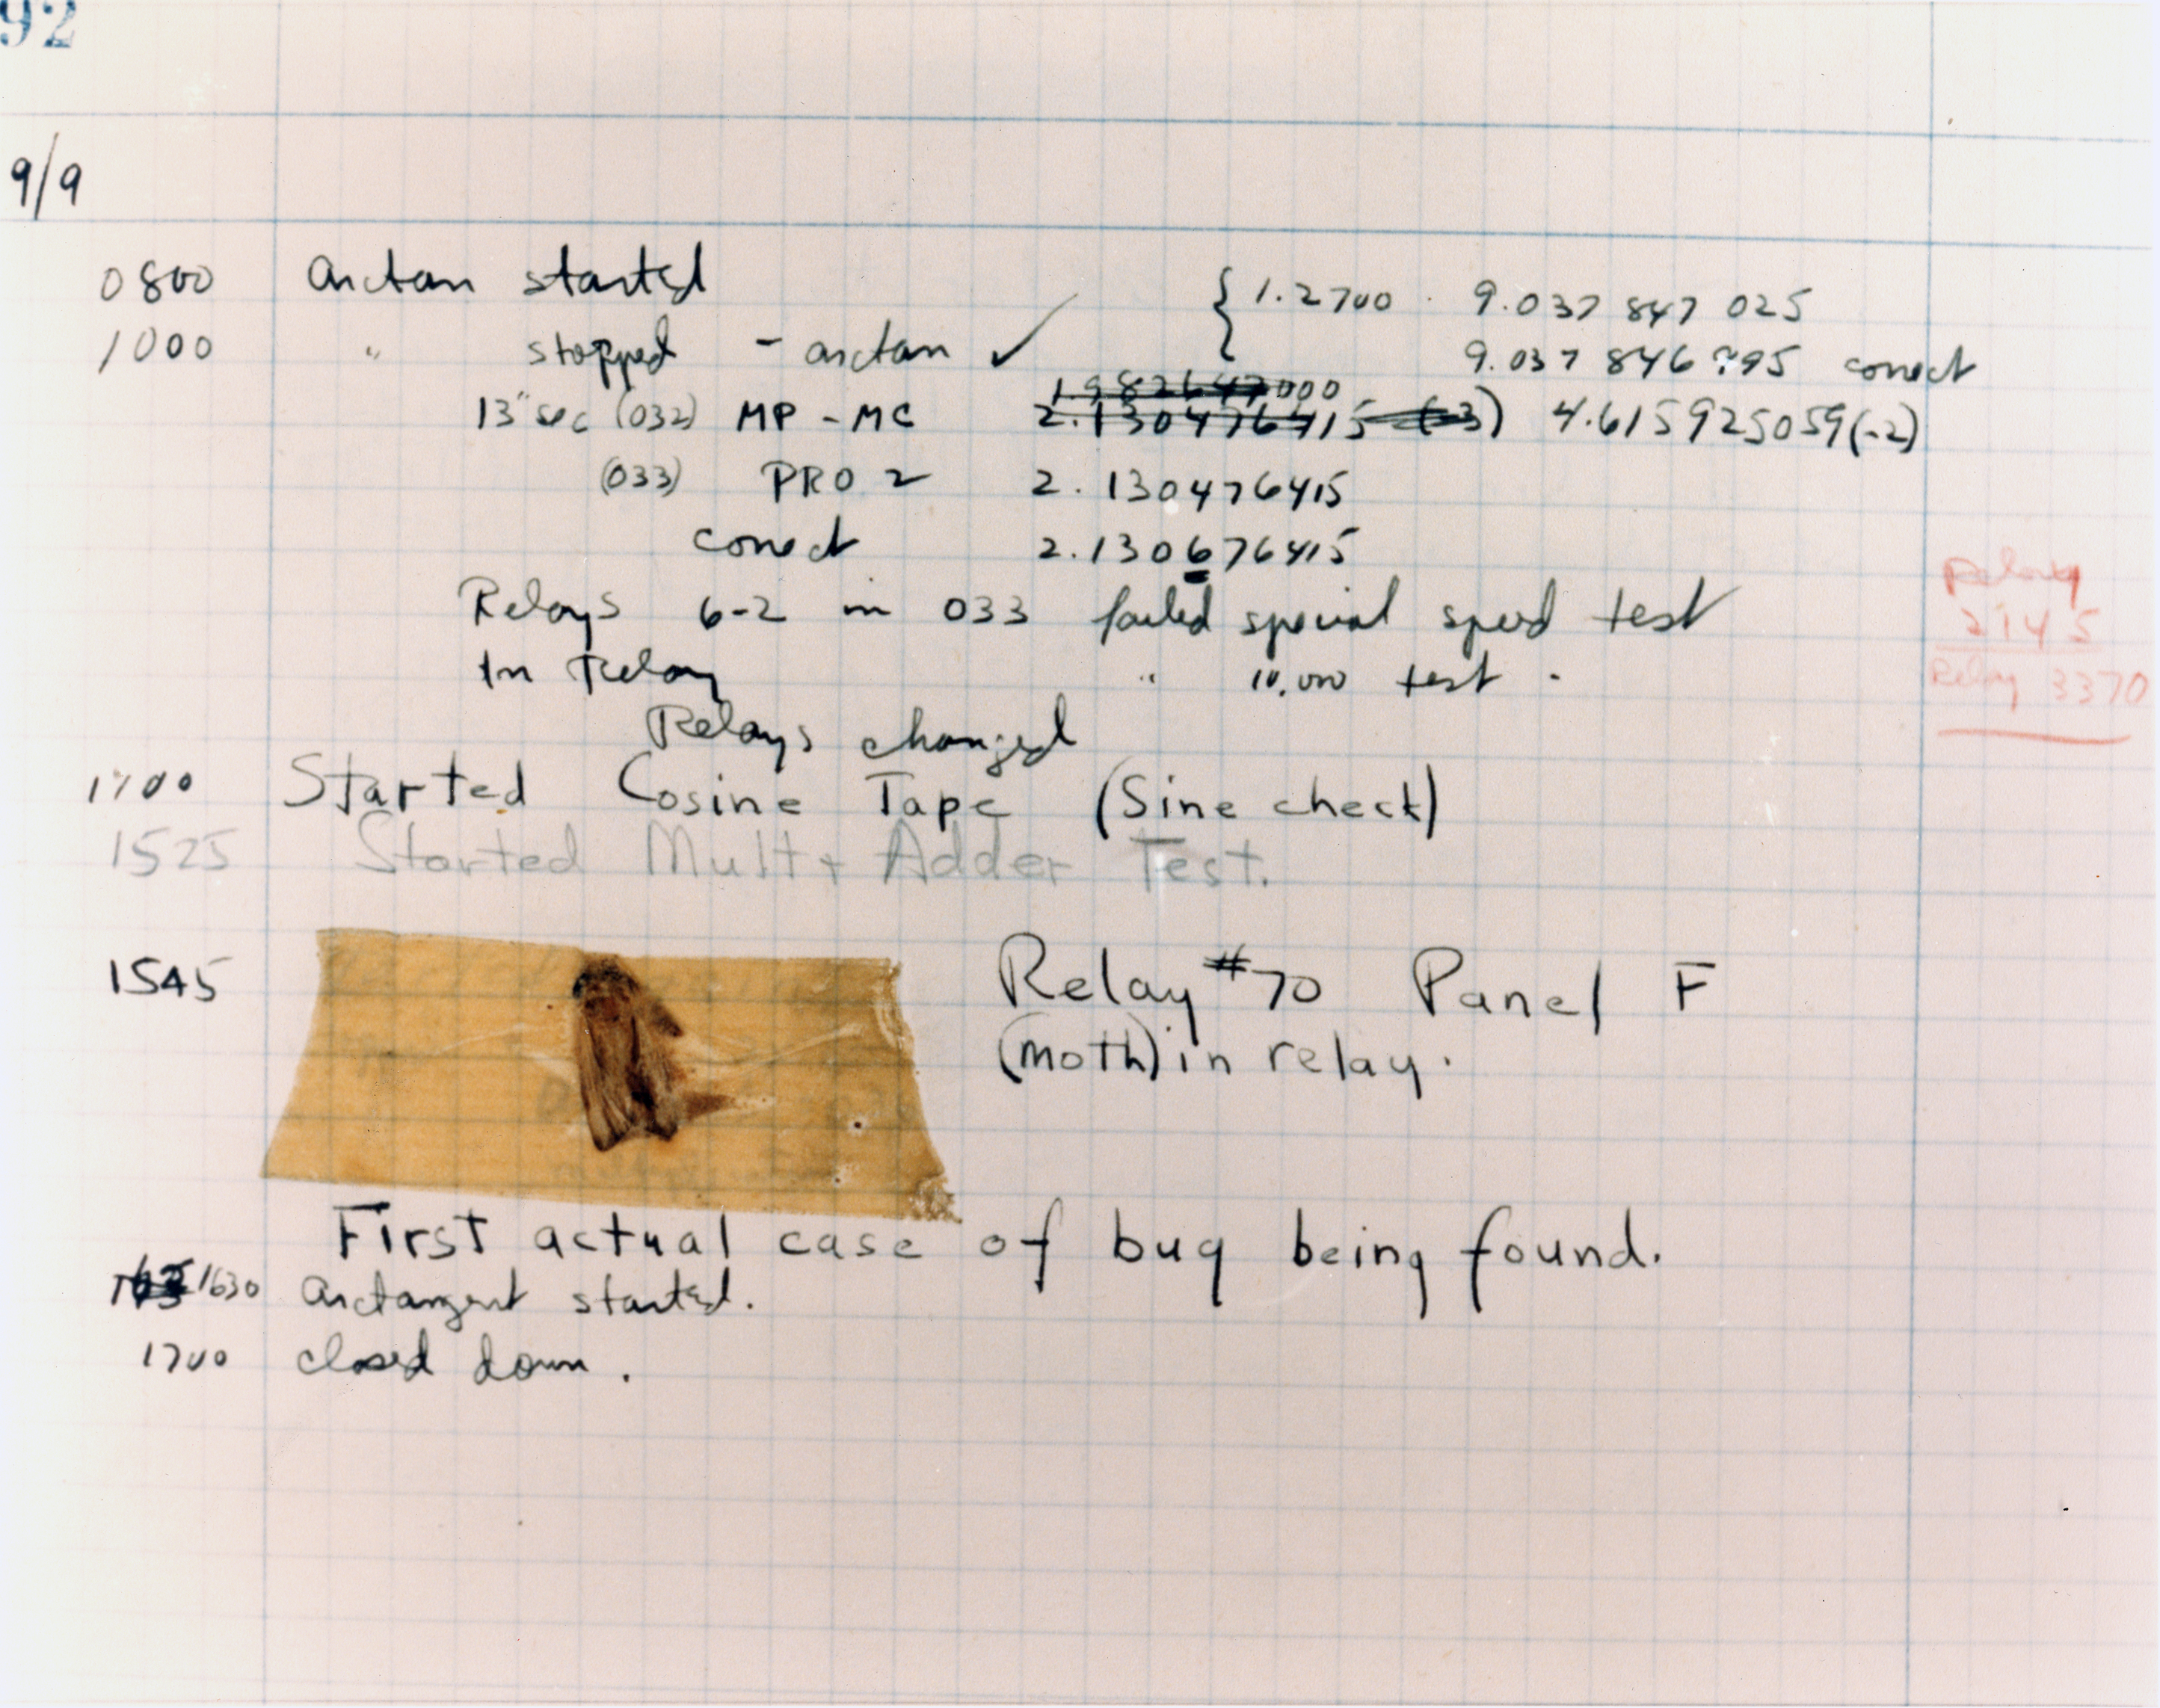
\includegraphics[scale=0.3]
    {./Presentations-pictures/Bug-found-1947.jpeg}

    \caption{Wpis w~księdze pracy komputera Mark~II z~$1947$ roku. Obok ćmy
      która utknęła w~jego wnętrzu zakłócając pracę, Hopper napisał
      „Pierwszy przypadek znalezienia prawdziwego robaka (ang.
      \textit{bug})”.}

  \end{figure}

\end{frame}
% ##################










% ######################################
\section{Podstawy działania kompilatora}
% ######################################



% ##################
\begin{frame}
  \frametitle{Prosty schemat działania kompilatora}


  \begin{figure}

    \begin{tikzpicture}[node distance=0.7]

      \node[diagram rectangle block] (Source code) at (0,0)
      {Kod źródłowy programu};

      \node[diagram block,below=of Source code] (Compiler)
      {Magia (kompilator)};

      \draw[thick diagram arrow] (Source code) -- (Compiler);



      \node[diagram rectangle block,below=of Compiler] (Assembly code)
      {Kod programu w~asemblerze};

      \draw[thick diagram arrow] (Compiler) -- (Assembly code);

    \end{tikzpicture}

    \caption{Ilustracja działania kompilatora~;).}


  \end{figure}

\end{frame}
% ##################





% ##################
\begin{frame}
  \frametitle{Schemat działania kompilatora}


  Kompilator to bardzo skomplikowany program, więc będziemy kolejne
  fazy jego działania odsłaniać po kolei. Zaczniemy od~tego, że~najpierw
  nasz kod źródłowy jest przetwarzany w~fazie analizy do reprezentacji
  pośredniej.





  \begin{textblock}{10.1}(1.4,3.7)

    \begin{figure}

      \begin{tikzpicture}[node distance=0.7]

        \node[diagram rectangle block] (Source code) at (0,0)
        {Kod źródłowy programu};

        \node[diagram block,right=of Source code] (Analitic phase)
        {Faza analizy};

        \draw[thick diagram arrow] (Source code) -- (Analitic phase);


        \node[diagram rectangle block,right=of Analitic phase] (IR)
        {Kod w~reprezentacji pośredniej};

        \draw[thick diagram arrow] (Analitic phase) -- (IR);


        \node[diagram block,below=of IR] (Synthesis phase) {Faza syntezy};

        \draw[thick diagram arrow] (IR) -- (Synthesis phase);


        \node[diagram rectangle block,left=of Synthesis phase]
        (Assembly code) {Kod programu w~asemblerze};

        \draw[thick diagram arrow] (Synthesis phase) -- (Assembly code);

      \end{tikzpicture}

      \caption{Bardziej poprawny opis działania kompilatora.}


    \end{figure}

  \end{textblock}

\end{frame}
% ##################





% #################
\begin{frame}
  \frametitle{Faza analizy}


  Pierwszym etapem działania kompilatora jest \textbf{faza analizy}. Proszę
  sobie przypomnieć, że~komputer rozumie tylko swój dialekt asemblera,
  nie zaś takie języki jak C~czy Python. Jak sama nazwa wskazuje, w~fazie
  analizy, kompilator poddaje nasz kod źródłowy odpowiedniej procedurze
  analizy, by zrozumieć jego sens. Dzięki uzyskanej wiedzy, kompilator
  generuje następnie kod zapisany w~odpowiedniej reprezentacji pośredniej.

  \textbf{Reprezentacja pośrednia}, \textsc{ir},
  ang.~\textit{intermidiate representation}, spotyka~się też
  rozwinięcie \textit{internal representation}. Jest to pewien język
  programowania, możemy o~nim myśleć jako o~„fikcyjnym” asemblerze.
  Fikcyjnym w~tym sensie, że~nie jest ważne, czy istnieje w~materialnym
  świecie procesor, który rozumiem ten język. Może istnieć, ale nie musi,
  to jest dla nas bez znaczenia. Dlaczego w~ogóle potrzebujemy
  wprowadzać~\textsc{ir}? Jednym z~powodów jest ograniczenie czasu
  kompilacji.

\end{frame}
% ##################





% ##################
\begin{frame}
  \frametitle{Problem wielokrotnej kompilacji}


  \begin{figure}

    \begin{tikzpicture}[node distance=0.7]

      \node[diagram rectangle block] (Source code A) at (0,0)
      {Kod źródłowy programu};

      \node[diagram block,below=of Source code A] (Compiler A)
      {Magia (kompilator)};

      \draw[thick diagram arrow] (Source code A) -- (Compiler A);



      \node[diagram rectangle block,below=of Compiler A] (Assembly code A)
      {Kod programu w~asm. x86};

      \draw[thick diagram arrow] (Compiler A) -- (Assembly code A);





      \begin{scope}[xshift=4cm]

        \node[diagram rectangle block] (Source code B) at (0,0)
        {Kod źródłowy programu};

        \node[diagram block,below=of Source code B] (Compiler B)
        {Magia (kompilator)};

        \draw[thick diagram arrow] (Source code B) -- (Compiler B);



        \node[diagram rectangle block,below=of Compiler B] (Assembly code B)
        {Kod programu w~asm. \textsc{arm} 32};

        \draw[thick diagram arrow] (Compiler B) -- (Assembly code B);

      \end{scope}





      \begin{scope}[xshift=8cm]

        \node[diagram rectangle block] (Source code C) at (0,0)
        {Kod źródłowy programu};

        \node[diagram block,below=of Source code C] (Compiler C)
        {Magia (kompilator)};

        \draw[thick diagram arrow] (Source code C) -- (Compiler C);



        \node[diagram rectangle block,below=of Compiler C] (Assembly code C)
        {Kod programu w~asm. AArch64};

        \draw[thick diagram arrow] (Compiler C) -- (Assembly code C);

      \end{scope}


    \end{tikzpicture}

    \caption{Jeśli ten sam program ma działać na komputerach z~różnymi
      typami procesorów, to musimy kilkakrotnie wykonać cały
      proces kompilacji.}


  \end{figure}

\end{frame}
% ##################





% ##################
\begin{frame}
  \frametitle{Wykorzystane reprezentacji pośredniej}

  \vspace{-0.5em}



  \begin{figure}

    \begin{tikzpicture}[node distance=0.7]

      \node[diagram rectangle block] (Source code) at (0,0)
      {Kod źródłowy programu};

      \node[diagram block,right=of Source code] (Analitic phase)
      {Faza analizy};

      \draw[thick diagram arrow] (Source code) -- (Analitic phase);



      \node[diagram rectangle block,right=of Analitic phase] (IR)
      {Kod programu w~\textsc{ir}};

      \draw[thick diagram arrow] (Analitic phase) -- (IR);


      \node[diagram block,below=of IR] (Back-end) {Faza syntezy};

      \draw[thick diagram arrow] (IR) -- (Back-end);


      \node[diagram rectangle block] (Assembly ARM 32) at (0,-5.2)
      {Kod programu w~asm. \textsc{arm} 32};

      \draw[thick diagram arrow] (Back-end) -- (Assembly ARM 32);


      \node[diagram rectangle block] (Assembly AArch64) at (3.9,-5.2)
      {Kod programu w~asm. AArch64};

      \draw[thick diagram arrow] (Back-end) -- (Assembly AArch64);


      \node[diagram rectangle block] (Assembly x86) at (6.8,-5.2)
      {Kod programu w~asm. x86};

      \draw[thick diagram arrow] (Back-end) -- (Assembly x86);



      \node[text width=10em] (Front-end description) at (2.8,-2)
      {$90\%$ procesu kompilacji wykonujemy do tego miejsca.};

      \draw[pointing arrow] (Front-end description) -- (IR);



      \node[text width=10em] (Back-end work description)
      at (0.5,-3.5) {Tutaj wykonujemy tylko pozostałe $10\%$.};

      \draw[pointing arrow] (Back-end work description) -- (3.3,-3.55);

    \end{tikzpicture}

    \caption{Przykład wykorzystanie~\textsc{ir}.}


  \end{figure}

\end{frame}
% ##################





% ##################
\begin{frame}
  \frametitle{Faza syntezy}


  W~fazie analizy wykonywane jest około $90\%$ całego procesu kompilacji
  (ta liczba jest mocno orientacyjna, ale na razie niech nam to wystarczy).
  W~wyniku tego z~języka źródłowego, takiego jak~C, powstaje reprezentacja
  pośrednia~(\textsc{ir}).

  Następnie przechodzimy do \textbf{fazy syntezy}, w~trakcie której na
  podstawie reprezentacji pośredniej jest \alert{syntezowany} odpowiedni
  kod w~danym dialekcie asemblera, który będziemy mogli następnie uruchomić
  na~konkretnym komputerze. Ten fakt wyjaśnia też nazwę „reprezentacja
  pośrednia”.

  Jak już mówiliśmy, reprezentacja pośrednia \textsc{ir} jest swego rodzaju
  fikcyjnym asemblerem. Ponieważ \textsc{ir} jest podobny do prawdziwych
  dialektów asemblera, tłumaczenie z~\textsc{ir} zajmuje mniej
  czasu kompilacji i~pochłania niewiele mocy obliczeniowej, niż kompilacja
  bezpośrednio z~języka takiego jak C do~\textsc{ir}.

\end{frame}
% ##################





% ##################
\begin{frame}
  \frametitle{Główne elementy kompilatora}

  \vspace{-0.5em}


  Część kompilatora odpowiedzialna za~fazę analizy nosi angielską
  nazwę \textbf{compiler front-end}, na polski tłumaczymy to jako
  „przód/front kompilatora”. Część kompilatora która na
  podstawie reprezentacji pośredniej tworzy właściwy kod asemblera nosi
  angielską nazwę \textbf{compiler back-end}. Po polsku zwykle mówimy „tył
  kompilatora”.





  \begin{textblock}{10.1}(1.4,3.7)

    \begin{figure}

      \begin{tikzpicture}[node distance=0.7]

        \node[diagram rectangle block] (Source code) at (0,0)
        {Kod źródłowy programu};

        \node[diagram block,right=of Source code] (Front-end)
        {Front kompilatora};

        \draw[thick diagram arrow] (Source code) -- (Front-end);


        \node[diagram rectangle block,right=of Front-end] (IR)
        {Kod w~reprezentacji pośredniej};

        \draw[thick diagram arrow] (Front-end) -- (IR);


        \node[diagram block,below=of IR] (Back-end) {Tył kompilatora};

        \draw[thick diagram arrow] (IR) -- (Back-end);


        \node[diagram rectangle block,left=of Back-end]
        (Assembly code) {Kod programu w~asemblerze};

        \draw[thick diagram arrow] (Back-end) -- (Assembly code);

      \end{tikzpicture}

      \caption{Ilustracja działania części kompilatora.}


    \end{figure}

  \end{textblock}

\end{frame}
% ##################










% ######################################
\section{Front kompilatora}
% ######################################



% ##################
\begin{frame}
  \frametitle{Schemat działania frontu kompilatora. Część~I}


  \begin{figure}

    \begin{tikzpicture}[node distance=0.7]

      \node[diagram rectangle block] (Source code) at (0,0)
      {Kod źródłowy programu};

      \node[diagram block,right=of Source code] (Lexer)
      {Lekser};

      \draw[thick diagram arrow] (Source code) -- (Lexer);


      \node[diagram rectangle block] (Symbols table) at (3.4,-2.3)
      {Tablica symboli};

      \draw[thick diagram arrow,color=red] (Lexer) -- (Symbols table);



      \node[diagram rectangle block,right=of Lexer] (Stream of tokens)
      {Strumień tokenów};

      \draw[thick diagram arrow] (Lexer) -- (Stream of tokens);


      \node[diagram block,below=of Stream of tokens] (Parser)
      {Parser};

      \draw[thick diagram arrow] (Stream of tokens) -- (Parser);


      \draw[thick diagram arrow] (Symbols table) -- (Parser);


      \node[diagram rectangle block,below=of Parser]
      (Syntax tree A) {Drzewo składniowe};

      \draw[thick diagram arrow] (Parser) -- (Syntax tree A);


      \node[diagram block,left=of Syntax tree A]
      (Semantic analizer) {Analizator semantyczny};

      \draw[thick diagram arrow] (Syntax tree A) --
      (Semantic analizer);


      \draw[thick diagram arrow] (Symbols table) -- (Semantic analizer);

      % \node[diagram rectangle block,below=of Parser]
      % (Semantic analizator) {Analizator semantyczny};

      % \draw[thick diagram arrow] (Parser) -- (Semantic analizator);


      \node[diagram rectangle block,left=of Semantic analizer]
      (Syntax tree B) {Zmodyfikowane drzewo składniowe};

      \draw[thick diagram arrow] (Semantic analizer) --
      (Syntax tree B);

    \end{tikzpicture}

    \caption{Działa frontu kompilatora, część~I.}


  \end{figure}

\end{frame}
% ##################





% ##################
\begin{frame}
  \frametitle{Schemat działania frontu kompilatora. Część~II}


  \begin{figure}

    \begin{tikzpicture}[node distance=0.7]

      \node[diagram rectangle block] (Syntax tree B) at (0,0)
      {Zmodyfikowane drzewo składniowe};

      \node[diagram block,right=of Syntax tree B] (Generator of IR)
      {Generacja reprezentacji pośredniej \textsc{ir}};

      \draw[thick diagram arrow] (Syntax tree B) -- (Generator of IR);


      \node[diagram rectangle block] (Symbols table) at (3.4,-2.3)
      {Tablica symboli};

      \draw[thick diagram arrow] (Symbols table) -- (Generator of IR);



      \node[diagram rectangle block,right=of Generator of IR]
      (IR) {Reprezentacja pośrednia \textsc{ir}};

      \draw[thick diagram arrow] (Generator of IR) -- (IR);

    \end{tikzpicture}

    \caption{Działa frontu kompilatora, część~II.}


  \end{figure}

\end{frame}
% ##################





% ##################
\begin{frame}
  \frametitle{Tył kompilatora}


  \begin{figure}

    \begin{tikzpicture}[node distance=0.7]

      \node[diagram rectangle block] (IR) at (0,0)
      {Reprezentacja pośrednia \textsc{ir}};

      \node[diagram block,right=of IR] (Optimalization of IR)
      {Optymalizacja reprezentacji pośredniej \textsc{ir}};

      \draw[thick diagram arrow] (IR) -- (Optimalization of IR);


      \node[diagram rectangle block] (Symbols table) at (3.4,-2.3)
      {Tablica symboli};

      \draw[thick diagram arrow] (Symbols table) -- (Optimalization of IR);



      \node[diagram rectangle block,right=of Generator of IR]
      (Modified IR) {Zmodyfikowany \textsc{ir}};

      \draw[thick diagram arrow] (Optimalization of IR) -- (Modified IR);


      \node[diagram block,below=of Modified IR]
      (Generation of assembly code) {Generowanie kodu asemblera};

      \draw[thick diagram arrow] (Modified IR) --
      (Generation of assembly code);

      \draw[thick diagram arrow] (Symbols table) --
      (Generation of assembly code);


      \node[diagram rectangle block,below=of Generation of assembly code]
      (Assembly code) {Kod assemblera};

      \draw[thick diagram arrow] (Generation of assembly code) --
      (Assembly code);


      \node[diagram block,left=of Assembly code]
      (Optimalization of assembly code) {Optymalizacja kodu assemblera};

      \draw[thick diagram arrow] (Assembly code) --
      (Optimalization of assembly code);

      \draw[thick diagram arrow] (Symbols table) --
      (Optimalization of assembly code);


      \node[diagram rectangle block,left=of Optimalization of assembly code]
      (Optimalized assembly code) {Zoptymalizowany kod assemblera};

      \draw[thick diagram arrow] (Optimalization of assembly code) --
      (Optimalized assembly code);

    \end{tikzpicture}

    \caption{Działa frontu kompilatora, część~II.}


  \end{figure}

\end{frame}
% ##################





% ##################
\begin{frame}
  \frametitle{Pedantyczny komentarz}

  Abstrakcja i~siła myślenia symbolicznego


  Warto zaznaczyć, że~normalne języki takie jak angielski, birmański,
  francuski, japoński, polski, etc., to obiekty o~trudnym do pojęcia
  poziomie złożoności, bo korzystają z nich ludzie, którzy są znacznie
  bardziej skomplikowanymi bytami niż komputery. Jak ktoś ma wątpliwości
  niech spróbuje najpierw przeczytać dwutomową książkę Bruce’a Albertsa
  et al. \textit{Podstawy biologii komórki}.

  Badanie normalnych języków nie jest przedmiotem informatyki, tylko
  filologii, lingwistyka, językoznawstwa i~sam nie wiem czego jeszcze,
  dlatego nie będziemy wnikać w~problemy z jakimi mierzą się te dziedziny.
  Będziemy jednak wybiórczo korzystać
  z~języka polskiego i~angielskiego by ilustrować problemy jakie napotykamy.
  Choć bowiem z punktu widzenia informatyki języki ludzkie są dużo bardziej
  skomplikowane niż C czy Python, to ponieważ są to \alert{nasze} języki
  których ciągle używamy, są dla nas łatwiejsze w zrozumieniu.

  % Dlatego proszę się nie przywiązywać zbytnio do takich rzeczy, jak
  % wyróżnianie leksemów języka polskiego, bo człowiek utknie na różnych
  % problemach spoza naszej działki. Jak to czy w zdaniu „Kot się przeciąga.”,
  % leksemem jest samo „się”, czy dopiero „Kot się”, a może „się przeciąga”?

\end{frame}
% ##################




% % ##################
% \begin{frame}
%   \frametitle{Prosty schemat działania kompilatora}

%   \vspace{-0.5em}



%   \begin{figure}

%     \begin{tikzpicture}[node distance=0.7]

%       \node[diagram rectangle block] (Source code) at (0,0)
%       {Kod źródłowy programu};

%       \node[diagram block,right=of Source code] (Front-end)
%       {Front kompilatora};

%       \draw[thick diagram arrow] (Source code) -- (Front-end);



%       \node[diagram rectangle block,right=of Front-end] (IR)
%       {Kod programu w~\textsc{ir}};

%       \draw[thick diagram arrow] (Front-end) -- (IR);


%       \node[diagram block,below=of IR] (Back-end) {Tył kompilatora};

%       \draw[thick diagram arrow] (IR) -- (Back-end);


%       \node[diagram rectangle block] (Assembly ARM 32) at (0,-5.2)
%       {Kod programu w~asm. \textsc{arm} 32};

%       \draw[thick diagram arrow] (Back-end) -- (Assembly ARM 32);


%       \node[diagram rectangle block] (Assembly AArch64) at (3.9,-5.2)
%       {Kod programu w~asm. AArch64};

%       \draw[thick diagram arrow] (Back-end) -- (Assembly AArch64);


%       \node[diagram rectangle block] (Assembly x86) at (6.8,-5.2)
%       {Kod programu w~asm. x86};

%       \draw[thick diagram arrow] (Back-end) -- (Assembly x86);



%       \node[text width=10em] (Front-end description) at (2.8,-2)
%       {$90\%$ procesu kompilacji wykonujemy do tego miejsca.};

%       \draw[pointing arrow] (Front-end description) -- (IR);



%       \node[text width=10em] (Back-end work description)
%       at (0.5,-3.5) {Tutaj wykonujemy tylko pozostałe $10\%$.};

%       \draw[pointing arrow] (Back-end work description) -- (3.3,-3.55);





%       % \end{scope}





%       % \begin{scope}[xshift=8cm]

%       %   \node[diagram rectangle block] (Source code C) at (0,0)
%       %   {Kod źródłowy programu};

%       %   \node[diagram block,below=of Source code C] (Compiler C)
%       %   {Magia (kompilator)};

%       %   \draw[thick diagram arrow] (Source code C) -- (Compiler C);



%       %   \node[diagram rectangle block,below=of Compiler C] (Assembly code C)
%       %   {Kod programu w~asm. AArch64};

%       %   \draw[thick diagram arrow] (Compiler C) -- (Assembly code C);

%       % \end{scope}


%     \end{tikzpicture}

%     \caption{Przykład wykorzystanie~\textsc{ir}.}


%   \end{figure}

% \end{frame}
% % ##################






% ##################
\begin{frame}
  \frametitle{Pedantyczny komentarz}


  % Warto zaznaczyć, że~normalne języki takie jak angielski, birmański,
  % francuski, japoński, polski, etc., to obiekty o~trudnym do pojęcia
  % poziomie złożoności, bo korzystają z nich ludzie, którzy są znacznie
  % bardziej skomplikowanymi bytami niż komputery. Jak ktoś ma wątpliwości
  % niech spróbuje najpierw przeczytać dwutomową książkę Bruce’a Albertsa
  % et al. \textit{Podstawy biologii komórki}.

  % Badanie normalnych języków nie jest przedmiotem informatyki, tylko
  % filologii i~językoznawstwa, dlatego nie będziemy wnikać w~problemy z
  % jakimi mierzą się te dziedziny. Będziemy jednak wybiórczo korzystać
  % z~języka polskiego i~angielskiego by ilustrować problemy jakie napotykamy.
  % Choć bowiem z punktu widzenia informatyki języki ludzkie są dużo bardziej
  % skomplikowane niż C czy Python, to ponieważ są to \alert{nasze} języki
  % których ciągle używamy, są dla nas łatwiejsze w zrozumieniu.

  Dlatego proszę się nie przywiązywać zbytnio do takich rzeczy, jak
  wyróżnianie leksemów języka polskiego, bo człowiek utknie na różnych
  problemach spoza naszej działki. Jak to czy w zdaniu „Kot się przeciąga.”,
  leksemem jest samo „się”, czy dopiero „Kot się”, a może „się przeciąga”?

\end{frame}
% ##################





% ##################
\begin{frame}
  \frametitle{Obliczenia w~zapisie numerycznym i~symbolicznym}


  $\displaystyle \frac{ 3.1415 }{ 18.849 } + \frac{ 3.1415 }{ 18.849 } +
  \frac{ 3.1415 }{ 18.849 } = \frac{ 6.283 }{ 18.849 } +
  \frac{ 3.1415 }{ 18.849 } = \frac{ 9.4245 }{ 18.849 } = \frac{ 1 }{ 2 }$

  \vspace{1em}


  $a = 3.1415$

  $\displaystyle \frac{ a }{ 6a } + \frac{ a }{ 6a } + \frac{ a }{ 6a } =
  \frac{ 1 } { 2 }$

  Schemat działania prawdziwego kompilatora.

  Kod źródłowy -> Lekser (analizator leksykalny) -> Strumień tokenów i
  tablica symboli -> Parser (analizator składniowy) -> Drzewo
  składniowe -> Analizator semantyczny -> Zoptymalizowane drzewo składniowe
  -> Generator kodu pośredniego -> IR, reprezentacja pośrednia ->
  Optymalizator kodu pośredniego -> Zoptymalizowany IR -> Generator
  asemblera -> Kod asemblera -> Optymalizacja asemblera ->
  Zoptymalizowany asembler

\end{frame}
% ##################





% % ##################
% \begin{frame}
%   \frametitle{Schemat działania prawdziwego kompilatora}


  % $\displaystyle \frac{ 3.1415 }{ 18.849 } + \frac{ 3.1415 }{ 18.849 } +
  % \frac{ 3.1415 }{ 18.849 } = \frac{ 6.283 }{ 18.849 } +
  % \frac{ 3.1415 }{ 18.849 } = \frac{ 9.4245 }{ 18.849 } = \frac{ 1 }{ 2 }$

  % \vspace{1em}


  % $a = 3.1415$

  % $\displaystyle \frac{ a }{ 6a } + \frac{ a }{ 6a } + \frac{ a }{ 6a } =
  % \frac{ 1 } { 2 }$

  % Kod źródłowy -> Lekser (analizator leksykalny) -> Strumień tokenów i
  % tablica symboli -> Parser (analizator składniowy) -> Drzewo
  % składniowe -> Analizator semantyczny -> Zoptymalizowane drzewo składniowe
  % -> Generator kodu pośredniego -> IR, reprezentacja pośrednia ->
  % Optymalizator kodu pośredniego -> Zoptymalizowany IR -> Generator
  % asemblera -> Kod asemblera -> Optymalizacja asemblera ->
  % Zoptymalizowany asembler

% \end{frame}
% % ##################




% ##################
\begin{frame}
  \frametitle{Schemat działania prawdziwego kompilatora}


  % $\displaystyle \frac{ 3.1415 }{ 18.849 } + \frac{ 3.1415 }{ 18.849 } +
  % \frac{ 3.1415 }{ 18.849 } = \frac{ 6.283 }{ 18.849 } +
  % \frac{ 3.1415 }{ 18.849 } = \frac{ 9.4245 }{ 18.849 } = \frac{ 1 }{ 2 }$

  % \vspace{1em}


  % $a = 3.1415$

  % $\displaystyle \frac{ a }{ 6a } + \frac{ a }{ 6a } + \frac{ a }{ 6a } =
  % \frac{ 1 } { 2 }$

  Kod źródłowy -> Lekser (analizator leksykalny) -> Strumień tokenów i
  tablica symboli -> Parser (analizator składniowy) -> Drzewo
  składniowe -> Analizator semantyczny -> Zoptymalizowane drzewo składniowe

  Niech „Azor” będzie imieniem konkretnego psa i weźmy zdanie \\
  „Azor wbiegł do pokoju.”
  Analiza leksykalna polega na rozbiciu tego zdania na części
  posiadające znaczenie: „Azor”, „wbiegł”, „do”, „pokoju”, „.”. Częścią
  znaczącą nie jest choćby „zor” czy „egł d”.

  Analiza składniowa polega na przypisaniu wyrazów do odpowiednich typów
  gramatycznych i~zbadanie czy razem tworzą dobrze zbudowane zdanie.
  „Azor” i „pokój” to rzeczowniki „wbiegł” to czasownik, „do” to nie
  pamiętam co (język polski to mój wróg), zaś „.” to znak interpunkcyjny.

\end{frame}
% ##################





% ##################
\begin{frame}
  \frametitle{????}


  % $\displaystyle \frac{ 3.1415 }{ 18.849 } + \frac{ 3.1415 }{ 18.849 } +
  % \frac{ 3.1415 }{ 18.849 } = \frac{ 6.283 }{ 18.849 } +
  % \frac{ 3.1415 }{ 18.849 } = \frac{ 9.4245 }{ 18.849 } = \frac{ 1 }{ 2 }$

  % \vspace{1em}


  % $a = 3.1415$

  % $\displaystyle \frac{ a }{ 6a } + \frac{ a }{ 6a } + \frac{ a }{ 6a } =
  % \frac{ 1 } { 2 }$

  W~języku polskim standardowe zdanie musi mieć podmiot będący rzeczownikiem
  i~orzeczenie będące czasownikiem.

  „Azor wbiegł do pokoju.” \\
  To jest dobrze zbudowane zdanie, bo ma podmiot „Azor” i~orzeczenie
  „wbiegł”.

  „Azor pokoju.” \\
  Od razu czuć, że to nie jest dobrze zbudowane zdanie, bo brak w~nim
  czasownika „wbiegł” (i „do”).

  „Do Azor wbiegł pokoju.” \\
  Zdanie ma podmiot i orzeczenie, ale od razu czuć, że coś tu jest nie tak.
  W~języku polskim „Do Azor” nie jest poprawnie zbudowany wyrażeniem,
  może jednak być „Do Azora podszedł inny pies.”.

  Język angielski ma znacznie bardziej sztywne reguły niż polski, więc
  tam to widać jeszcze lepiej

  % Kod źródłowy -> Lekser (analizator leksykalny) -> Strumień tokenów i
  % tablica symboli -> Parser (analizator składniowy) -> Drzewo
  % składniowe -> Analizator semantyczny -> Zoptymalizowane drzewo składniowe

  % Niech „Azor” będzie imieniem konkretnego psa i weźmy zdanie \\
  % „Azor wbiegł do pokoju.”
  % Analiza leksykalna polega na rozbiciu tego zdania na części
  % posiadające znaczenie: „Azor”, „wbiegł”, „do”, „pokoju”, „.”. Częścią
  % znaczącą nie jest choćby „zor” czy „egł d”.

  % Analiza składniowa polega na przypisaniu wyrazów do odpowiednich typów
  % gramatycznych i~zbadanie czy razem tworzą dobrze zbudowane zdanie.
  % „Azor” i „pokój” to rzeczowniki „wbiegł” to czasownik, „do” to nie
  % pamiętam co (język polski to mój wróg), zaś „.” to znak interpunkcyjny.

\end{frame}
% ##################





% % ##################
% \begin{frame}
%   \frametitle{Schemat działania prawdziwego kompilatora}


%   % $\displaystyle \frac{ 3.1415 }{ 18.849 } + \frac{ 3.1415 }{ 18.849 } +
%   % \frac{ 3.1415 }{ 18.849 } = \frac{ 6.283 }{ 18.849 } +
%   % \frac{ 3.1415 }{ 18.849 } = \frac{ 9.4245 }{ 18.849 } = \frac{ 1 }{ 2 }$

%   % \vspace{1em}


%   % $a = 3.1415$

%   % $\displaystyle \frac{ a }{ 6a } + \frac{ a }{ 6a } + \frac{ a }{ 6a } =
%   % \frac{ 1 } { 2 }$

%   Kod źródłowy -> Lekser (analizator leksykalny) -> Strumień tokenów i
%   tablica symboli -> Parser (analizator składniowy) -> Drzewo
%   składniowe -> Analizator semantyczny -> Zoptymalizowane drzewo składniowe

%   Niech „Azor” będzie imieniem konkretnego psa i weźmy zdanie „Azor wbiegł
%   do pokoju”.   Zdanie „Pies wbiegł do pokoju.” dzieli się na leksemy „Pies”, „wbiegł”,
%   „do”, „pokoju”, „.”, gdyż każdy z~nich posiada określony sens. Fragmenty
%   tego zdania, które nie są leksemami to choćby „zor”, „iegł d” czy „pok”.

% \end{frame}
% % ##################





% % ##################
% \begin{frame}
%   \frametitle{Pedantyczny komentarz}




% Abstrakcja i~siła myślenia symbolicznego


  % Warto zaznaczyć, że~normalne języki takie jak angielski, birmański,
  % francuski, japoński, polski, etc., to obiekty o~trudnym do pojęcia
  % poziomie złożoności, bo korzystają z nich ludzie, którzy są znacznie
  % bardziej skomplikowanymi bytami niż komputery. Jak ktoś ma wątpliwości
  % niech spróbuje najpierw przeczytać dwutomową książkę Bruce’a Albertsa
  % et al. \textit{Podstawy biologii komórki}.

  % Badanie normalnych języków nie jest przedmiotem informatyki, tylko
  % filologii, lingwistyka, językoznawstwa i~sam nie wiem czego jeszcze,
  % dlatego nie będziemy wnikać w~problemy z jakimi mierzą się te dziedziny.
  % Będziemy jednak wybiórczo korzystać
  % z~języka polskiego i~angielskiego by ilustrować problemy jakie napotykamy.
  % Choć bowiem z punktu widzenia informatyki języki ludzkie są dużo bardziej
  % skomplikowane niż C czy Python, to ponieważ są to \alert{nasze} języki
  % których ciągle używamy, są dla nas łatwiejsze w zrozumieniu.

  % Dlatego proszę się nie przywiązywać zbytnio do takich rzeczy, jak
  % wyróżnianie leksemów języka polskiego, bo człowiek utknie na różnych
  % problemach spoza naszej działki. Jak to czy w zdaniu „Kot się przeciąga.”,
  % leksemem jest samo „się”, czy dopiero „Kot się”, a może „się przeciąga”?

% \end{frame}
% % ##################





% ##################
\begin{frame}
  \frametitle{Lekser}


  Dla nas dzielenie zdań normalnego języka w ten sposób jest tak naturalne,
  że o tym nawet nie myślimy, ale komputer jest tępy i by móc jakoś
  zrozumieć dany program, musi najpierw go podzielić na leksemy za pomocą
  odpowiedniego, bardzo mocno sprecyzowanego określonego algorytmu.
  Chyba, że~akurat natrafimy na
  \colorhref{http://www.catb.org/jargon/html/N/nasal-demons.html}
  {demony nasala}.

\end{frame}
% ##################





% ##################
\begin{frame}
  \frametitle{Parser}


  Zdanie „Pies wbiegł do pokoju.” dzieli się na leksemy „Pies”, „wbiegł”,
  „do”, „pokoju”, „.”, gdyż każdy z~nich posiada określony sens. Fragmenty
  tego zdania, które nie są leksemami to choćby „es”, „iegł d” czy „pok”.

  Dla nas dzielenie zdań normalnego języka w ten sposób jest tak naturalne,
  że o tym nawet nie myślimy, ale komputer jest tępy i by móc jakoś
  zrozumieć dany program, musi najpierw go podzielić na leksemy za pomocą
  odpowiedniego, bardzo mocno sprecyzowanego określonego algorytmu.
  Chyba, że~akurat natrafimy na
  \colorhref{http://www.catb.org/jargon/html/N/nasal-demons.html}
  {demony nasala}.

\end{frame}
% ##################











% ##################
\begin{frame}
  \frametitle{??????}


  Kod źródłowy -> Lekser (analizator leksykalny) -> Strumień tokenów i
  tablica symboli -> Parser (analizator składniowy) -> Drzewo
  składniowe -> Analizator semantyczny -> Zoptymalizowane drzewo składniowe

  Pierwszą częścią kompilatora jest \textbf{lekser}, znany też jako
  analizator leksykalnym. Jego zadaniem jest podzielenie programu
  komputerowego na jednostki znaczące, zwane \textbf{leksemami}, lub
  mniej formalnie \textbf{tokenami}. Ogólną zasadę można zrozumieć na
  prostym przykładzie z~języka polskiego.

  „Azor wbiegł do pokoju.” dzieli się na leksemy [„Azor”, „wbiegł”, „do”,
  „pokoju”, „.”]. Leksemy dzielimy dwa typy: symbole abstrakcyjne
  i~identyfikatory. Identyfikatory są chyba prostsze do zrozumienia.

\end{frame}
% ##################





% ##################
\begin{frame}
  \frametitle{??????}


  Identyfikator to pewien symbol, który identyfikuje zewnętrzny obiekt.
  Imię każdego z nas jest mniej więcej tym czym jest identyfikator
  w~informatyce. Każdemu identyfikatorowi lekser przyporządkowuje
  \textbf{token} w~postaci: \\
  $( \text{nazwa}, \text{pozycja w tablicy symboli} )$

  Identyfikatorem jest „Azor”, dla którego lekser generuje token
  $( \text{id}, 1 )$, gdzie „id” oznacza, że jest to identyfikator (ang.
  \textit{identifier}), a~$1$ to numer pozycji w~tablicy symboli.

  \begin{center}

    \begin{tabular}{|c|c|c|c|c|}

      \hline
      1 & Azor & pies & kundel & przyjazny \\
      \hline
    \end{tabular}

  \end{center}

\end{frame}
% ##################





% ##################
\begin{frame}
  \frametitle{?????}


  Drugim typem tokenu jest \textbf{symbol abstrakcyjny}. W~skrócie symbol
  abstrakcyjny oznacza sam siebie. Nie jest nazwą żadnego zewnętrznego
  obiektu, zwykle jest nazwą pewnej czynności, operacji matematycznej, etc.
  Do ich zapisu będziemy używać oznaczeń $\langle symbol \rangle$.

  „Azor wbiegł do pokoju.” -> [„Azor”, „wbiegł”, „do”, „pokoju”, „.”]

  „Azor” to identyfikator. Przyjmiemy, że „pokój” też jest identyfikatorem
  który oznacza jakieś konkretne pomieszczenie. Symbole abstrakcyjne to
  „wbiegł”, „do” oraz „.”.

  Lekser przekształci nam „Azor wbiegł do pokoju.” na \\
  $( \text{id}, 1 ) \langle \text{wbiegł} \rangle \langle \text{do} \rangle ( \text{id}, 2 )$.

  \begin{center}

    \begin{tabular}{|c|c|c|c|c|}

      \hline
      1 & Azor & pies & kundel & przyjazny \\
      2 & pokoju & sypialnia & ulica & miasto \\
      \hline
    \end{tabular}

  \end{center}

\end{frame}
% ##################





% % ######################################
% \section{??????}
% % ######################################






































% % ##################
% \begin{frame}
%   \frametitle{?????}



% \end{frame}
% % ##################





% % ##################
% \begin{frame}
%   \frametitle{???????}




% \end{frame}
% % ##################





% % ##################
% \begin{frame}
%   \frametitle{?????}




% \end{frame}
% % ##################





% % ##################
% \begin{frame}
%   \frametitle{?????}



% \end{frame}
% % ##################






% % ##################
% \begin{frame}
%   \frametitle{?????}




% \end{frame}
% % ##################





% % ##################
% \begin{frame}
%   \frametitle{?????}




% \end{frame}
% % ##################





% % ##################
% \begin{frame}
%   \frametitle{??????}



% \end{frame}
% % ##################





% % ##################
% \begin{frame}
%   \frametitle{??????}




% \end{frame}
% % ##################





% % ##################
% \begin{frame}
%   \frametitle{???????}



% \end{frame}
% % ##################






% % ##################
% \begin{frame}
%   \frametitle{??????}



% \end{frame}
% % ##################





% % ##################
% \begin{frame}
%   \frametitle{??????}




% \end{frame}
% % ##################





% % ##################
% \begin{frame}
%   \frametitle{???????}



% \end{frame}
% % ##################





% % ##################
% \begin{frame}
%   \frametitle{??????}



% \end{frame}
% % ##################





% % ##################
% \begin{frame}
%   \frametitle{??????}



% \end{frame}
% % ##################





% % ##################
% \begin{frame}
%   \frametitle{?????}



% \end{frame}
% % ##################





% % ##################
% \begin{frame}
%   \frametitle{??????}



% \end{frame}
% % ##################





% % ##################
% \begin{frame}
%   \frametitle{???????}



% \end{frame}
% % ##################





% % ##################
% \begin{frame}
%   \frametitle{????}



% \end{frame}
% % ##################





% % ##################
% \begin{frame}
%   \frametitle{?????}




% \end{frame}
% % ##################





% % ##################
% \begin{frame}
%   \frametitle{??????}




% \end{frame}
% % ##################





% % ##################
% \begin{frame}
%   \frametitle{?????}




% \end{frame}
% % ##################





% % ##################
% \begin{frame}
%   \frametitle{?????}




% \end{frame}
% % ##################





% % ##################
% \begin{frame}
%   \frametitle{?????}





% \end{frame}
% % ##################





% % ##################
% \begin{frame}
%   \frametitle{?????}





% \end{frame}
% % ##################





% % ##################
% \begin{frame}
%   \frametitle{?????}




% \end{frame}
% % ##################





% % ##################
% \begin{frame}
%   \frametitle{?????}





% \end{frame}
% % ##################





% % ##################
% \begin{frame}
%   \frametitle{?????}





% \end{frame}
% % ##################





% % ##################
% \begin{frame}
%   \frametitle{??????}





% \end{frame}
% % ##################





% % ##################
% \begin{frame}
%   \frametitle{??????}




% \end{frame}
% % ##################





% % ##################
% \begin{frame}
%   \frametitle{????}






% \end{frame}
% % ##################





% % ##################
% \begin{frame}
%   \frametitle{?????}





% \end{frame}
% % ##################





% % ##################
% \begin{frame}
%   \frametitle{????}




% \end{frame}
% % ##################










% % ######################################
% \appendix
% % ######################################






% % % ##################
% % \jagiellonianendslide{Dziękuję za~uwagę.}
% % % ##################










% % ######################################
% \section{?????}
% % ######################################



% % ##################
% \begin{frame}
%   \frametitle{?????}




% \end{frame}
% % ##################





% ##################
% \begin{frame}
%   \frametitle{?????}




% \end{frame}
% ##################





% ##################
% \begin{frame}
%   \frametitle{?????}




% \end{frame}
% ##################





% ##################
% \begin{frame}
%   \frametitle{?????}




% \end{frame}
% ##################





% ##################
% \begin{frame}
%   \frametitle{?????}



% \end{frame}
% ##################
















% ####################################################################

% End of the document
\end{document}
